\chapter{Technical Specification}\label{ch:technical-specification}
\section{Requirements for IDPs}\label{sec:requirements-for-idps}
The \gls{IDP} is a critical component of the remote signing solution,
since identification and authentication is delegated to it.
Furthermore, if the \gls{IDP} is not carefully selected and vetted,
the most significant security advantage of our solution as compared to existing services,
like Adobe Document Cloud or Swisscom All-In Signing Service,
the distribution of trust,
may be compromised.

This is why the \gls{IDP} used with any instance of this signing service must be carefully selected,
and it must fulfil at least the following requirements,
in addition to the requirements specified by \gls{ETSI}~\cite{etsicarequirements}.

All of the requirements specified must be met in order for qualified signatures to be emitted.
For an explanation on what qualified signatures are, please see~\ref{subsubsec:qualifiedsignature}.

\subsection{Independence of IDP and Signing Service}\label{subsec:organisational-and-financial-independence}
The \gls{IDP} and the organisation responsible for it must be independent from the organisation responsible for the signing service and vice versa
It must not be the same company, or conglomerate, or even the same owner of two companies,
that own or operate these services;
because otherwise there may be a single stakeholder able to influence or even control both.
This must never happen as it would compromise the distribution of trust.

\subsection{Enrollment and Identity Proofing Requirements}\label{subsec:enrollment-and-identity-proofing-requirements}
The \gls{IDP} is required to identify and register users at \gls{IAL3} as defined by \gls{NIST}~\cite{nistregister}.
In practice, this means that physical presence is required for identification,
and two pieces of strong physical proof of identification has to be presented,
such as a passport as well as a drivers' licence.
For a complete list of requirements, please see the relevant \gls{NIST} publication~\cite{nistregister}.

\subsection{Authentication and Lifecycle Management Requirements}\label{subsec:authentication-and-lifecycle-management-requirements}
The \gls{IDP} is required to authenticate users at \gls{AAL3} as defined by \gls{NIST}~\cite{nistauthenticate}.
This level of authentication requires the use of a multi-factor hardware crypto device,
such as a MobileID \gls{SIM} card with a key protected by a \gls{PIN} not shorter than six digits
(something you have, plus something you know).
The use of software multi-factor crypto devices is allowed as well, but only in combination with additional factors.
For a complete list of requirements, please see the relevant \gls{NIST} publication~\cite{nistauthenticate}.

\subsection{Requirements for Advanced Electronic Signatures}\label{subsec:requirements-for-advanced-electronic-signatures}
The requirements specified in~\ref{subsec:enrollment-and-identity-proofing-requirements}~and~\ref{subsec:authentication-and-lifecycle-management-requirements} apply to qualified electronic signatures.
For advanced electronic signatures, \gls{AAL2} is sufficient.
The \gls{AAL} required by the signing service to emit the desired signature level can be specified to the \gls{IDP}~\cite[Section 2]{oidc-core-spec},
and is subsequently confirmed by the \gls{IDP} in the field \texttt{acr} of the \gls{JWT} \texttt{id\_token}.
If the \gls{IDP} does not confirm the required \gls{AAL}, the signing process is aborted.
Since the \texttt{id\_token} is included in the signature file, anyone can verify the \gls{AAL} confirmation by the \gls{IDP}.

\subsection{Use of proper X.509 Certificates and Chains for Signing JWTs}\label{subsec:use-of-x.509-for-signing-jwts}
The \gls{IDP} is required to sign the \gls{JWT} \texttt{id\_tokens} using proper X.509 certificates
signed by a trusted \gls{CA}, and is required to publish the complete certificate chain in its \gls{JWKS}
in the field \texttt{x5c} as specified in~\cite[RFC 7515, Section 4.1.6]{rfc7515}.
This \gls{JWKS} along with optional revocation information for \gls{LTV} can then be embedded into the signature file
by the signing service upon signature creation, and checked by the verifier, even offline.

\subsubsection{Reason for Requirement}
The use of X.509 is permitted by the \gls{JWS} standard~\cite[Section 5.1.6]{rfc7515} but not required for use with \gls{OIDC},
which is why we require it explicitly here.
Since a \gls{JWT} is a \gls{JWS}~\cite[Section 1]{rfc7519},
and a \gls{JWS} is used with a \gls{JWK}~\cite{rfc7517} stored in a \gls{JWKS},
and a \gls{JWKS} allows the use of keys other than X.509 certificates that are part of a certificate chain issued by a trusted \gls{CA},
this presents us with a problem.

Upon signature verification, the verifier needs to check whether the \texttt{id\_token} embedded into the signature really was issued by a trusted \gls{IDP}.
It verifies this by checking whom the \gls{JWT} \texttt{id\_token} was signed by.
If the verifier didn't check this, any valid \gls{JWT} could be placed into the signature and the link between the signer identity assertion and the data signed would be broken (or could be forged).

This verification is performed as described in~\cite[Section 7.2]{rfc7519} by using the \gls{JWKS} issued by the \gls{IDP}.
However, this \gls{JWKS} might contain plain public keys, not signed by any \gls{CA}~\footnote{For an example of a \gls{JWKS} using plain \gls{RSA} keys not signed by a \gls{CA}, see \url{https://www.googleapis.com/oauth2/v3/certs}.}.
If that \gls{JWKS} is embedded into the signature,
the verifier is able to confirm which key in the \gls{JWKS} was used in signing the \gls{JWT},
but there would be no way for the verifier to confirm that the \gls{JWKS} embedded into the signature
is authentic, that it really is the one used by the \gls{IDP}.
An attacker could embed an \texttt{id\_token} and a matching \gls{JWKS} into a signature file,
and the verifier would accept it.

There's an obvious solution for this: the verifier simply fetches the \gls{JWKS} from the \gls{IDP}
at verification time (over \gls{TLS}) and uses the keys contained in it to verify the \gls{JWT} \texttt{id\_token}.
As easy as this solution sounds, unfortunately it comes with two undesirable consequences:
\begin{enumerate}
    \item The verifier can no longer function offline. Embedding the \gls{JWKS} is useless as the verifier has no way of checking whom it was issued by.
    \item When the \gls{IDP} rotates the keys in the~\gls{JWKS}, which it will sooner or later,
    and no longer publishes the old keys used for signing the \texttt{id\_token} embedded into the signature,
    verification of the \texttt{id\_token}'s \gls{JWS} signature
    will no longer be possible, and thus the signature will be invalidated.
\end{enumerate}

This is why we require the use of proper X.509 certificates and chains for signing the \gls{JWT} \texttt{id\_token}.





\section{Protocol}\label{sec:protocol}

In this section, we provide an explanation of the protocol and the values used in it.

The protocol of our signing service consists of five main phases:

\begin{itemize}
    \item Pre-Login (see~\ref{subsec:pre-login})
    \item Login (see~\ref{subsec:login})
    \item Post-Login (see~\ref{subsec:post-login})
    \item Signature Generation (see~\ref{subsec:signature-generation})
    \item Signature Verification (see~\ref{subsec:signature-verification})
\end{itemize}

For a high-level overview of these phases, see figure~\ref{fig:highlevelprotocoloverview}.

\begin{figure}
    \begin{center}
        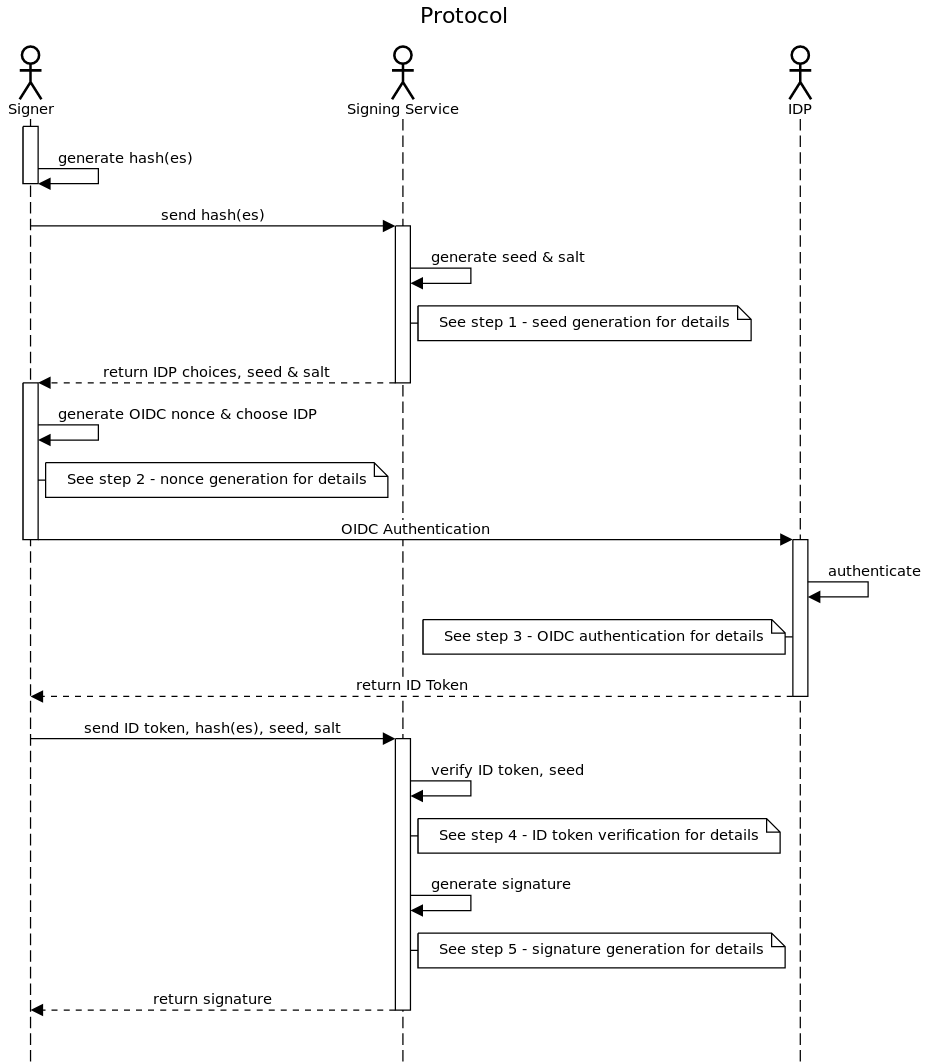
\includegraphics[scale=0.5]{images/protocol_signature_generation_high_level.png}
        \caption{High-level protocol overview}
        \label{fig:highlevelprotocoloverview}
    \end{center}
\end{figure}

\subsection{Pre-Login}\label{subsec:pre-login}
In this phase the signer provides a list of hashes to signing service
(this list may consist of just one entry in case the signer wishes to sign a single document).

Then, the signing service generates a random \texttt{seed}.

\[ seed = random() \]

This \texttt{seed}, together with a static \texttt{secret} known to the server only,
is used to calculate the key that is used to generate a \gls{HMAC}
of the sorted list\footnote{The list has to be sorted,
otherwise the same hash values in a different order would produce different \gls{HMAC}s.} of hashes.
The key is calculated using a \gls{HKDF} as specified in RFC~5869~\cite{rfc5869}.

\[ hmacKey = HKDF(seed, staticServerSecret) \]

From the key obtained from the \gls{HKDF} and the document hashes,
a salt value is derived by using a \gls{HMAC} as specified in RFC~2104~\cite{rfc2104}.

\[ salt = HMAC(hmacKey, sorted(hashes)) \]

Next, the nonce is calculated by masking each hash with the salt by using a \gls{HMAC},
and hashing this list with a secure hash algorithm~\cite{nistsha}.


\[ nonce = H(\{\ HMAC(salt, h) \ \ \forall \ h \in sorted(hashes)\ \}) \]

The nonce needs to be derived from the list of salted hashes because
only the salted hashes will be included in the signature file.


\paragraph{Purpose of the salt}
The salt is used to mask the document hashes in the \gls{OIDC} nonce from the \gls{IDP}.
This way the \gls{IDP} cannot learn whether two people sign the same document(s).
If we wouldn't salt the hashes, the \gls{OIDC} nonce would be the same for the same sorted list of hashes,
and the \gls{IDP} could detect when two people sign the same document(s).

While someone could argue that the IDP server learning about different people signing the same document
isn't much of a security problem, we want to ensure that each involved party is given the absolute minimum
of information necessary for them to fulfil their role\footnote{as specified in the non-functional requirements, "Protection of Information"}.

In addition to shielding the hashes from the \gls{IDP},
the salt masks the document hashes from recipients of multi-file signatures.
When multiple files are signed at once, all of the hashes are included in the resulting signature file.
However, since someone could receive only a subset of the files that were signed together,
they could learn the document hashes of the other files.
(For example, a company signing a thousand invoices at once but sending each customer only their invoice.)

Again, this shouldn't be a significant problem but again, we don't want to allow this.
So we include only the salted hashes in the signature file, and the salt itself.

Since the verifier is in possession of the document(s), they can calculate their respective hashes,
and then derive the salted hash(es) themselves since the salt is included in the signature file.
Then they can check whether their document hash(es) are in the list of salted hashes.
This way, they can verify their document(s) without learning anything about the other documents,
not even their hash values.

\paragraph{Purpose of the seed}
The seed is necessary in order to obtain a different \gls{HMAC} key for every request
despite using the same static secret on the server,
and in order to strengthen the \gls{HKDF} as recommended in RFC~5869~\cite[Section 3.1]{rfc5869}.
Furthermore, the seed is used as a \gls{CSRF} protection mechanism without the need for the server to keep any state.
If no such \texttt{seed} were used for generating the salt,
the signing server would be forced to keep the \gls{CSRF} token in memory and link it to the users session,
in order to be able to check whether the hashes or the salt were replaced somewhere in the \gls{OIDC} authentication implicit flow
(and as such, establishing the secure link between the document hashes and the authentication).
If the signing server didn't verify this,
it would allow for skipping the Pre-Login step (see~\ref{subsec:pre-login})
and proceeding directly to the Post-Login step (\ref{subsec:post-login}) as seen from the signing service.

The server then returns a list of \gls{IDP} choices as well as the \texttt{seed} and the \texttt{salt} to the client.

For a sequence diagram of this phase, see figure~\ref{fig:seedgenerationstep}.

\begin{figure}
    \begin{center}
        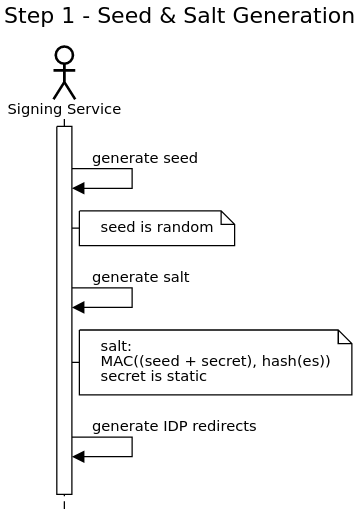
\includegraphics[scale=0.5]{images/protocol_step1_seed_generation.png}
        \caption{Seed generation step}
        \label{fig:seedgenerationstep}
    \end{center}
\end{figure}

\subsection{Login}\label{subsec:login}
TODO update graphic: no client-side generating anything because no one likes to write javascript
For a graphical representation of this, see figure~\ref{fig:noncegenerationstep}.

Having received a list of \gls{IDP}s from the server, the client chooses an \gls{IDP} and follows the link.
The user then authenticates with the \gls{IDP} and receives their ID token as seen in figure~\ref{fig:oidcauthenticationstep}.

\begin{figure}
    \begin{center}
        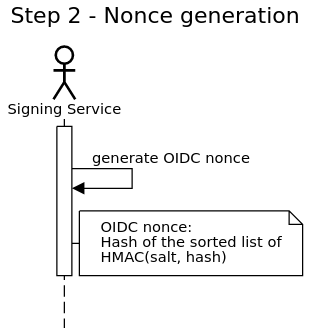
\includegraphics[scale=0.5]{images/protocol_step2_nonce_generation.png}
        \caption{Nonce generation step}
        \label{fig:noncegenerationstep}
    \end{center}
\end{figure}

\begin{figure}
    \begin{center}
        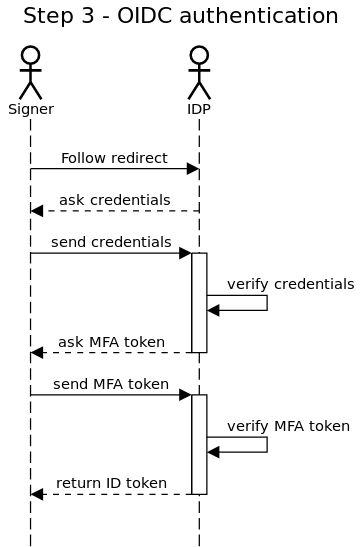
\includegraphics[scale=0.5]{images/protocol_step3_oidc_authentication.png}
        \caption{OIDC authentication step}
        \label{fig:oidcauthenticationstep}
    \end{center}
\end{figure}

\subsection{Post-Login}\label{subsec:post-login}
As shown in figure~\ref{fig:tokenverificationstep},
the client sends the ID token, the list of hashes, the \texttt{seed} and the \texttt{salt} to the signing service.
The signing service then verifies the \texttt{salt}, OIDC nonce and ID token as described in~\ref{subsubsec:verificationhashesseedsalt}.
After this step, the \texttt{seed} is not used anymore and should be discarded.


\subsubsection{Verification of hashes, seed and salt}\label{subsubsec:verificationhashesseedsalt}
Upon receiving a well-formed request in the format described in~\ref{subsubsec:signrequest},
the signing server performs no fewer than the following checks:
\begin{enumerate}
    \item Verifying the id\_token as described in~\cite[Section~7.2]{rfc7519}
    \item Checking the length of the seed and salt values
    \item Checking that the salt and nonce match the calculation described in~\ref{subsec:pre-login}
\end{enumerate}
These verifications are paramount to the safety of the system.

\begin{figure}
    \begin{center}
        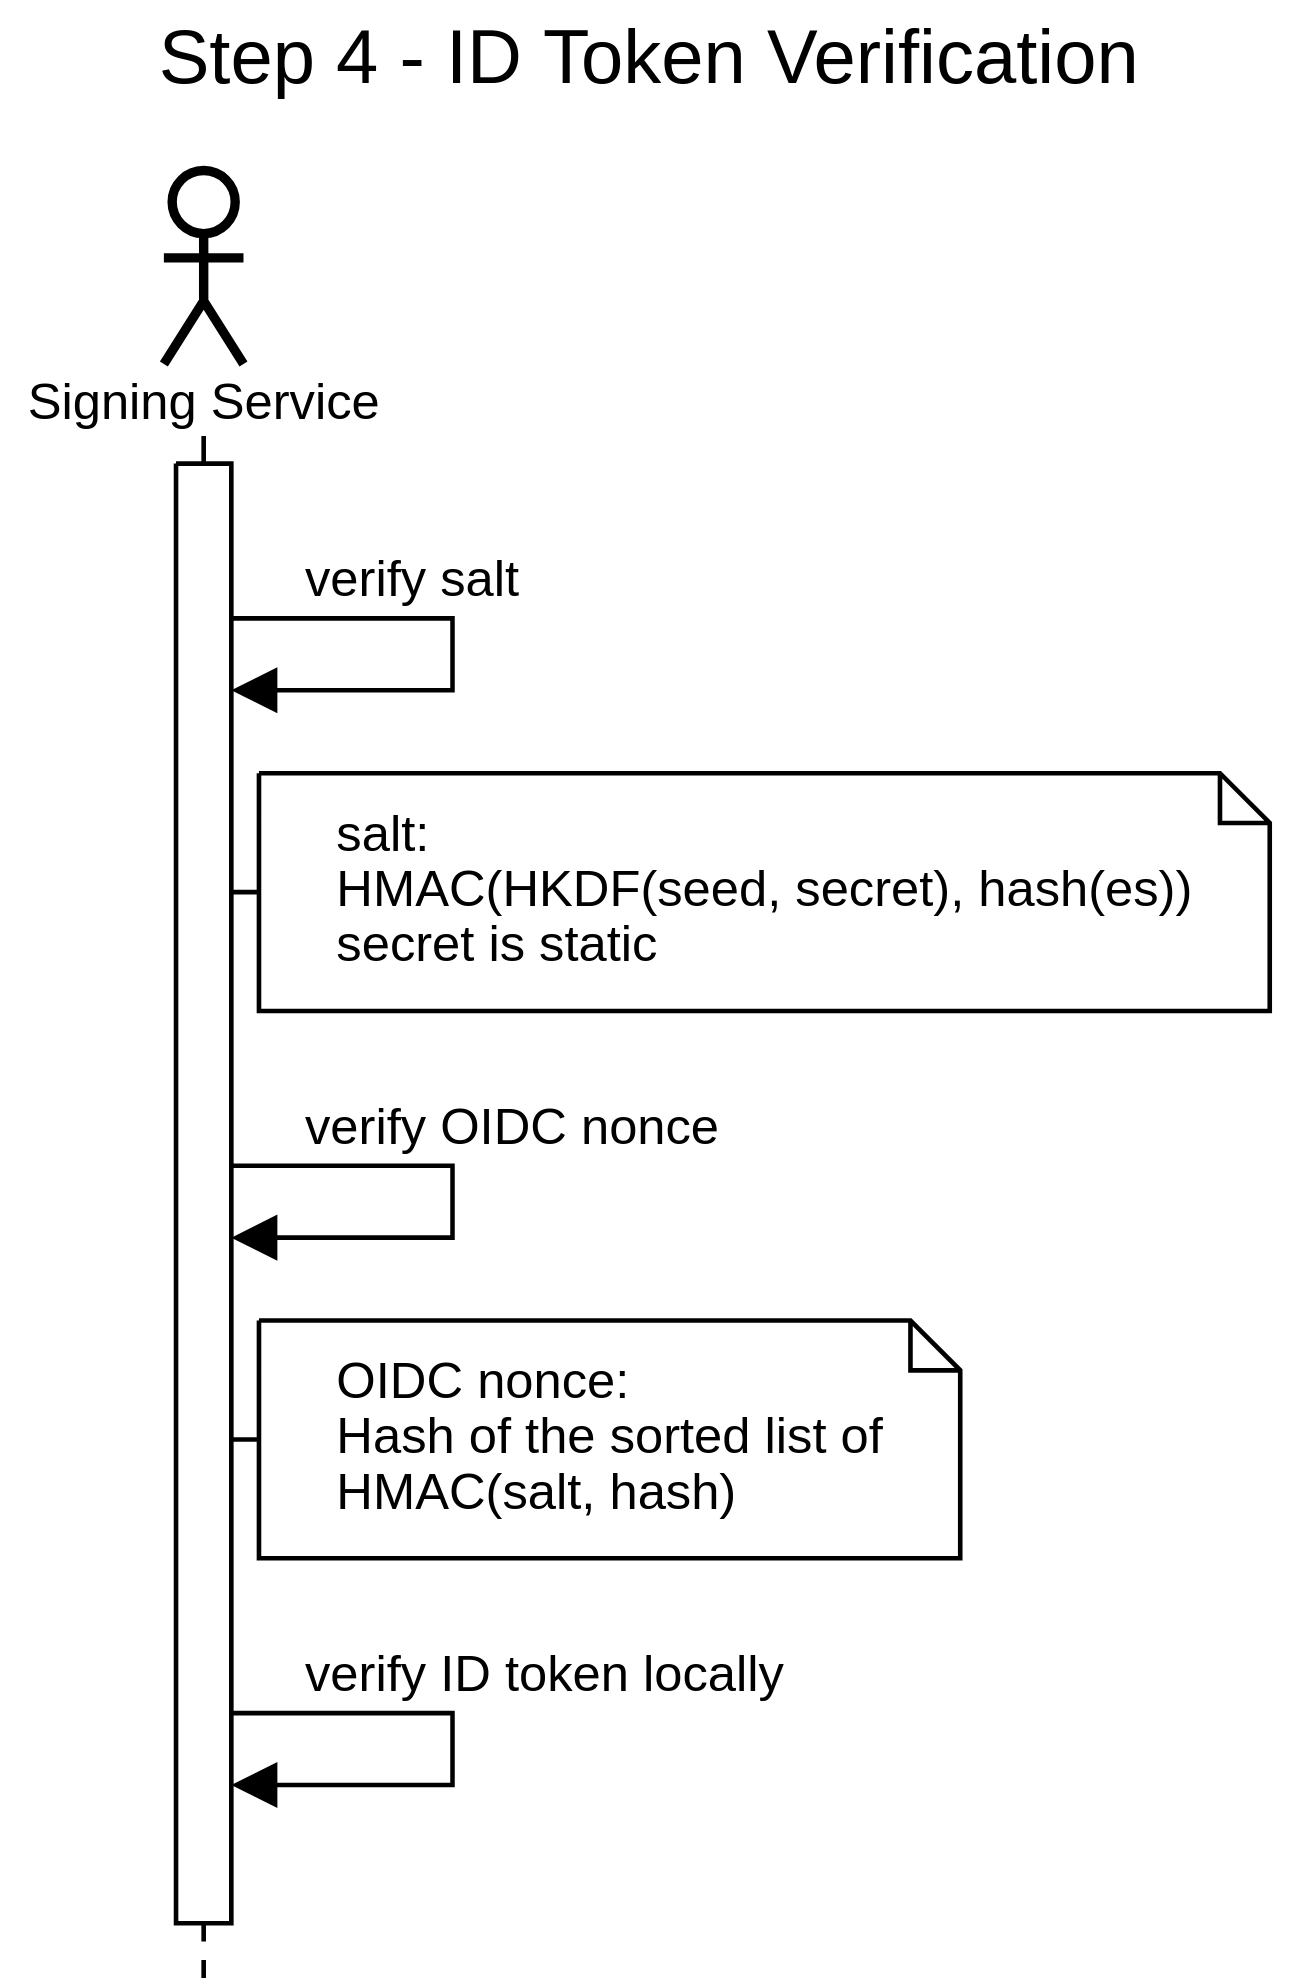
\includegraphics[scale=0.5]{images/protocol_step4_id_token_verification.png}
        \caption{Token verification step}
        \label{fig:tokenverificationstep}
    \end{center}
\end{figure}

\subsection{Signature Generation}\label{subsec:signature-generation}
The signing server requests a new signing key from the \gls{HSM}, which in turn generates a private key and returns a \gls{CSR}.
This \gls{CSR} is sent to the \gls{CA} where it is signed and the signed certificate returned.

Each hash is then submitted to the \gls{HSM} to be signed by the signing key.

Then, for each hash an intermediate signature file consisting of the signed hash,
the ID token, the \texttt{salt} and a sorted list of all other salted hashes is created.
The hash of this file is sent to a \gls{TSA} where a signed timestamp is created and returned.

Finally, the signed timestamp, and all the certificate chains,
\gls{OCSP} responses and \gls{CRL}s of the involved parties,
is added to signature file, which is then returned to the user.

TODO update this figure since we no longer loop
See figure~\ref{fig:signaturegenerationstep} for a sequence diagram of this process.

\begin{figure}
    \begin{center}
        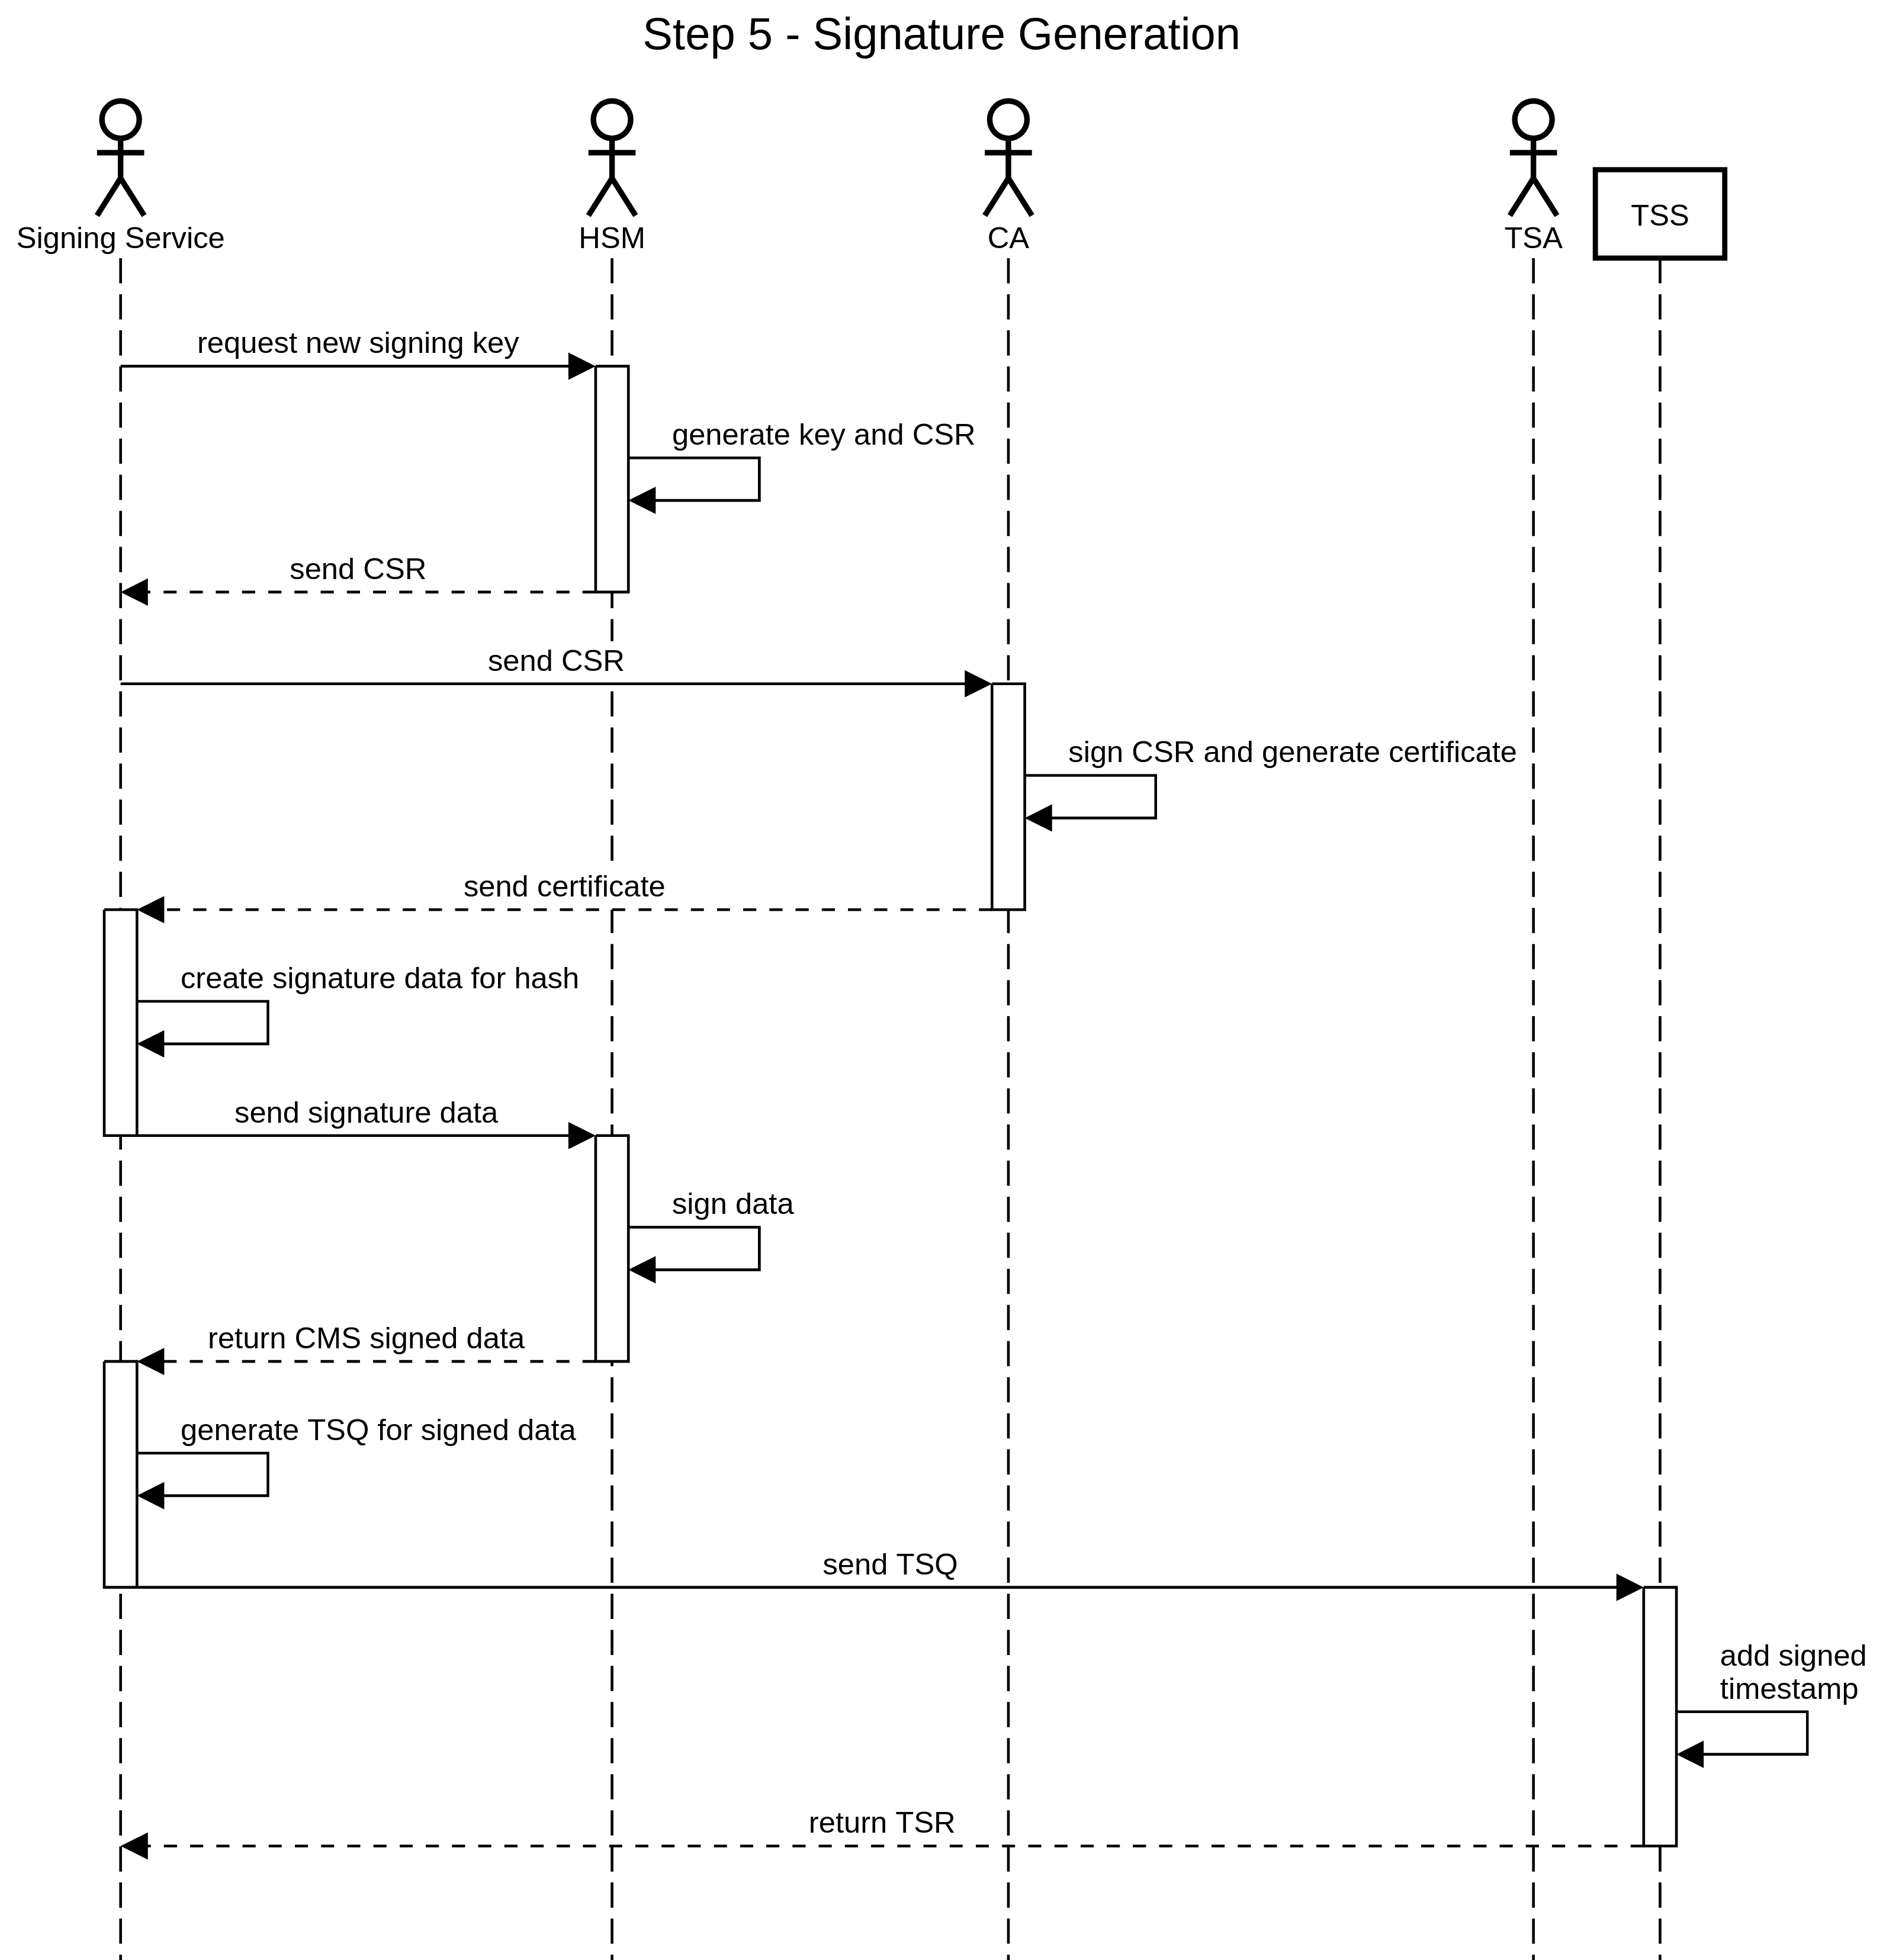
\includegraphics[scale=0.45]{images/protocol_step5_signature_generation.png}
        \caption{Signature generation step}
        \label{fig:signaturegenerationstep}
    \end{center}
\end{figure}

\subsection{Signature Verification}\label{subsec:signature-verification}

The signature verification can either be online (figure~\ref{fig:onlinesignatureverificationprotocol})
or offline (figure~\ref{fig:offlinesignatureverificationprotocol}).

For online verification, the user simply uploads the list of hashes and the signature file to the verification service.

\begin{figure}
    \begin{center}
        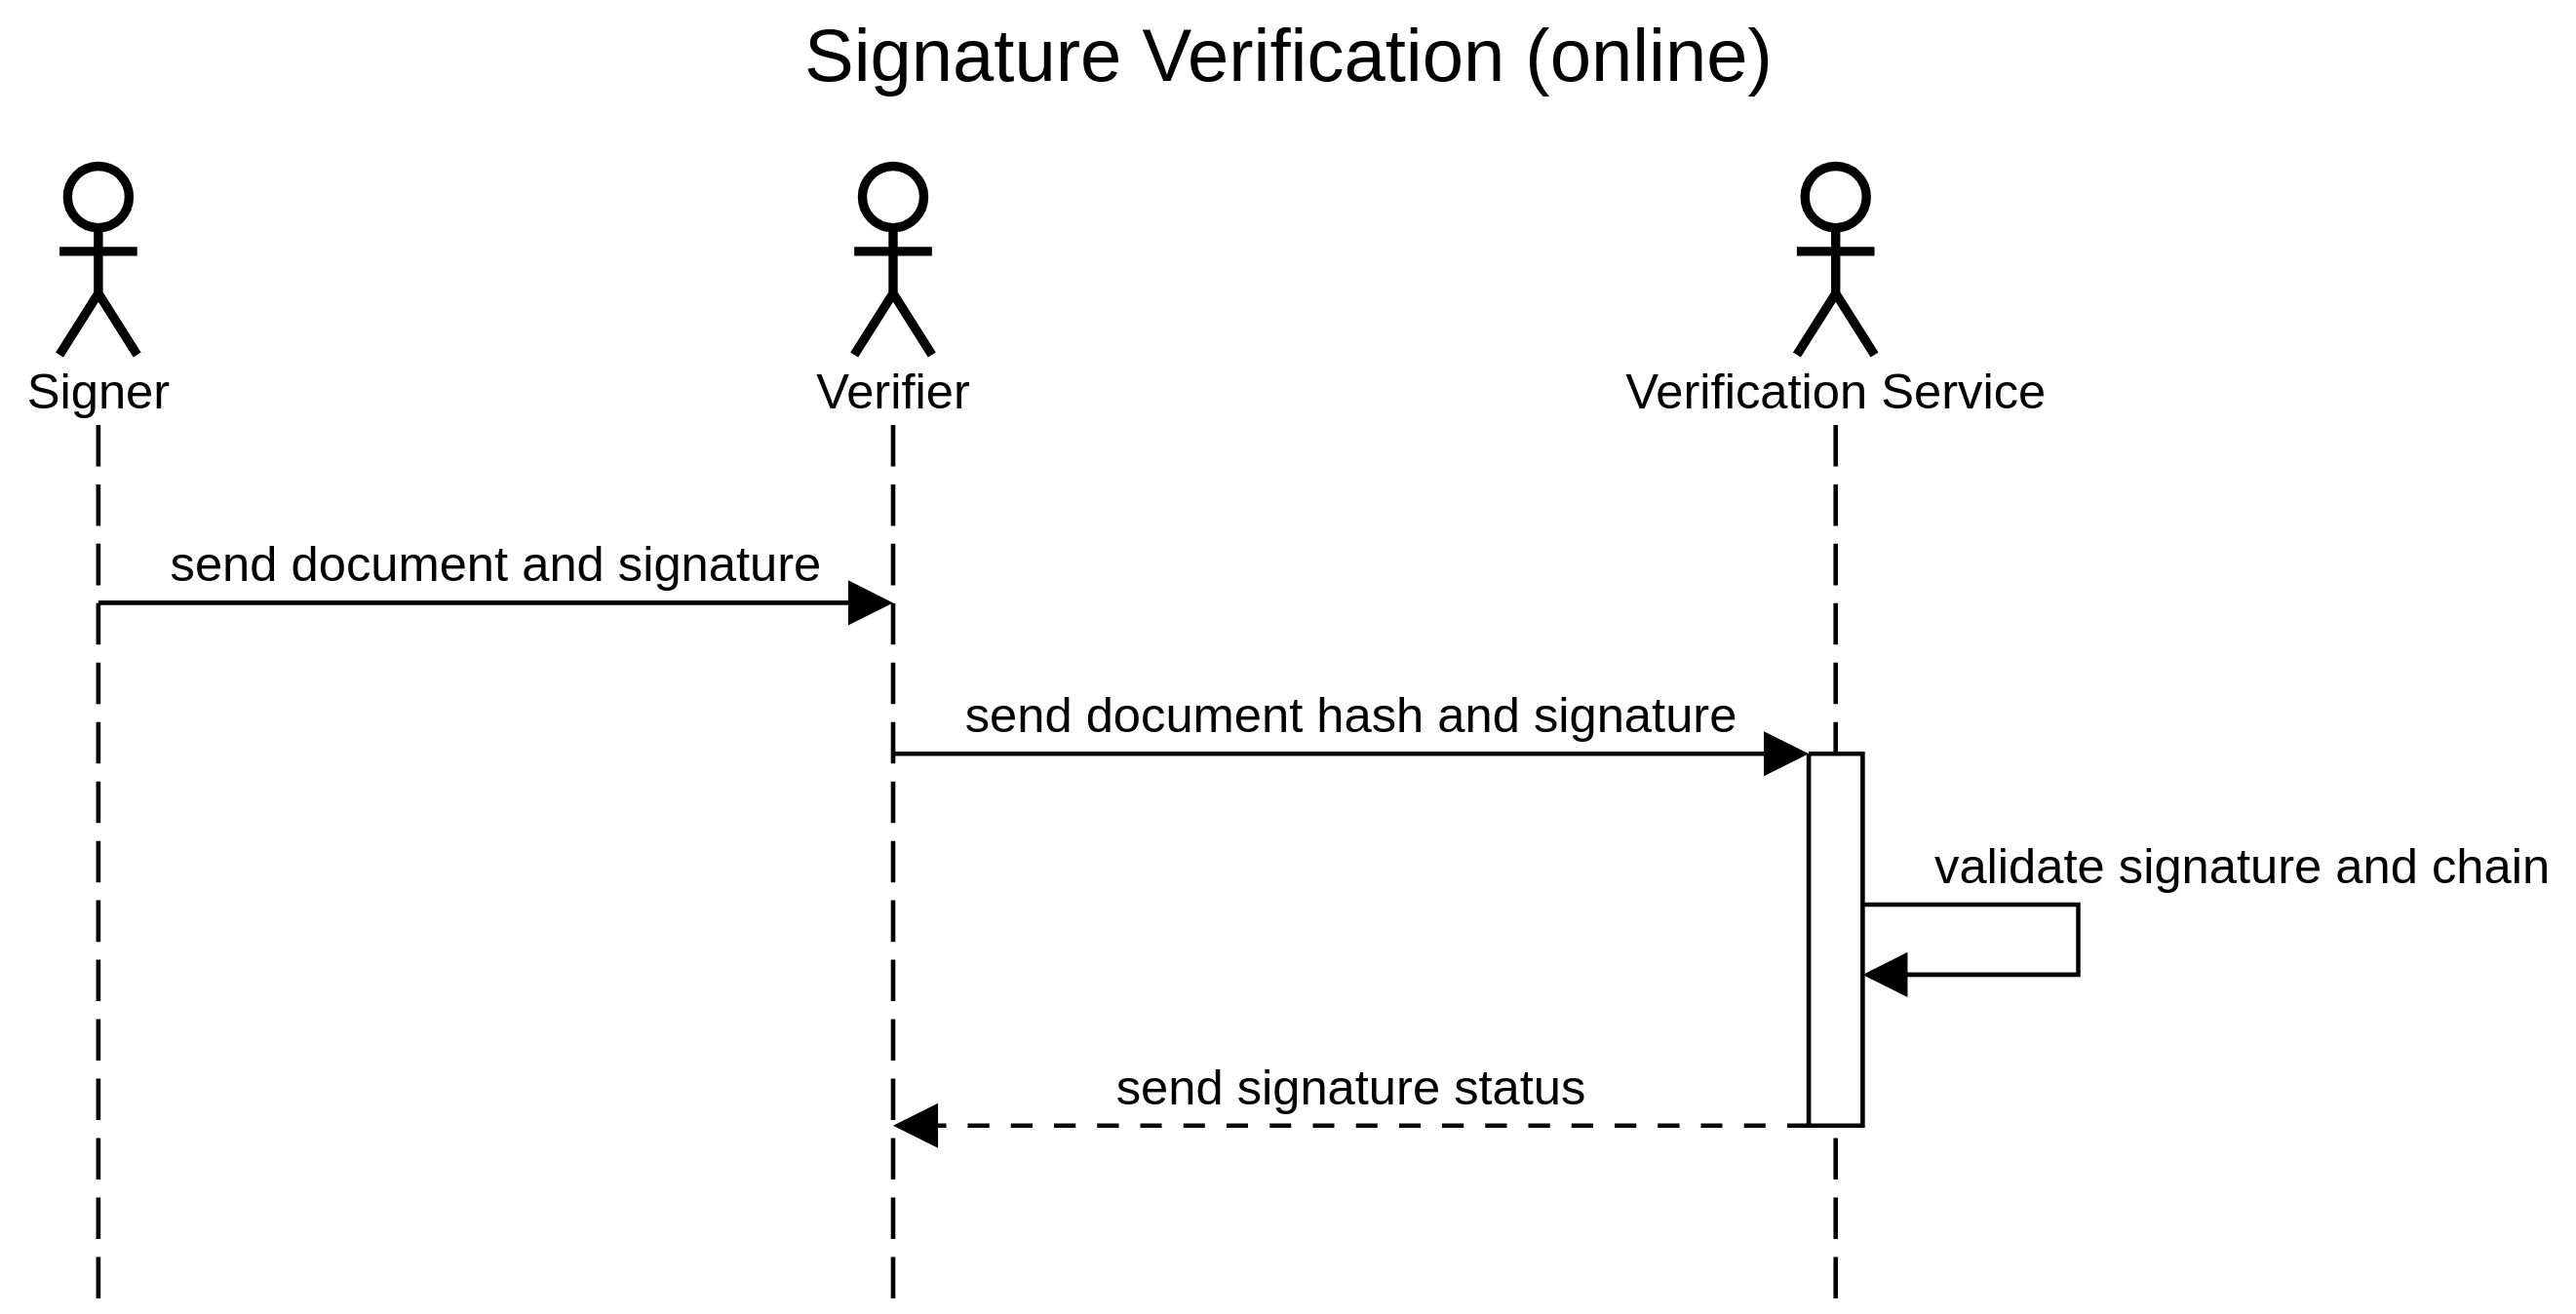
\includegraphics[scale=0.5]{images/protocol_online_verification_high_level.png}
        \caption{Online Signature Verification Protocol}
        \label{fig:onlinesignatureverificationprotocol}
    \end{center}
\end{figure}

For the offline verification, the user downloads the verification programme and starts it.
Then, they upload the list of hashes and signature file just as if they were using online verification,
but to their own copy of the verification service running on their computer without needing any network connection
instead of a remote verification service.

\begin{figure}
    \begin{center}
        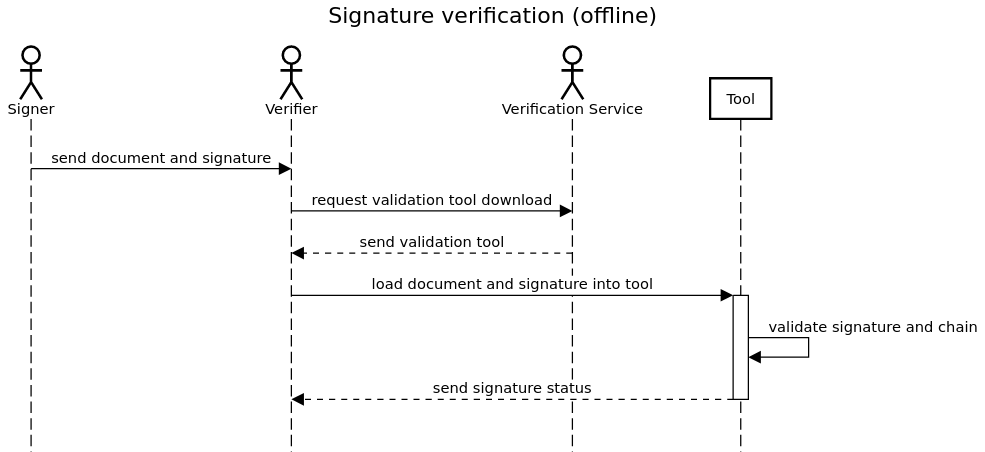
\includegraphics[scale=0.5]{images/protocol_offline_verification_high_level.png}
        \caption{Offline Signature Verification Protocol}
        \label{fig:offlinesignatureverificationprotocol}
    \end{center}
\end{figure}

To verify a signature,
the verifier first needs to verify the chain of signed timestamps and their respective \gls{CA} chains (figure~\ref{fig:timestampverificationstep}).

\begin{figure}
    \begin{center}
        % TODO update this figure since we no longer loop
        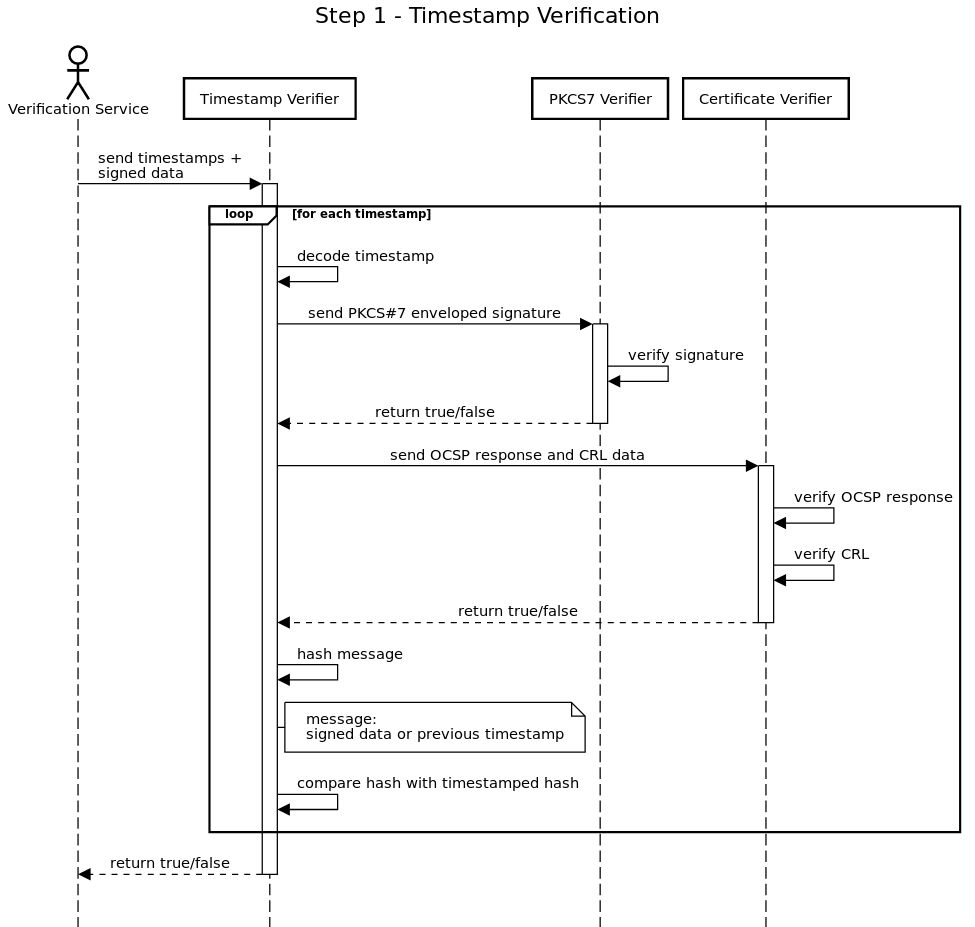
\includegraphics[scale=0.5]{images/protocol_verification_step1_timestamp.png}
        \caption{Timestamp verification step}
        \label{fig:timestampverificationstep}
    \end{center}
\end{figure}

The signature itself can then be verified (figure~\ref{fig:signaturegenerationstep}), along with
the certificate chain for the signing certificate.

\begin{figure}
    \begin{center}
        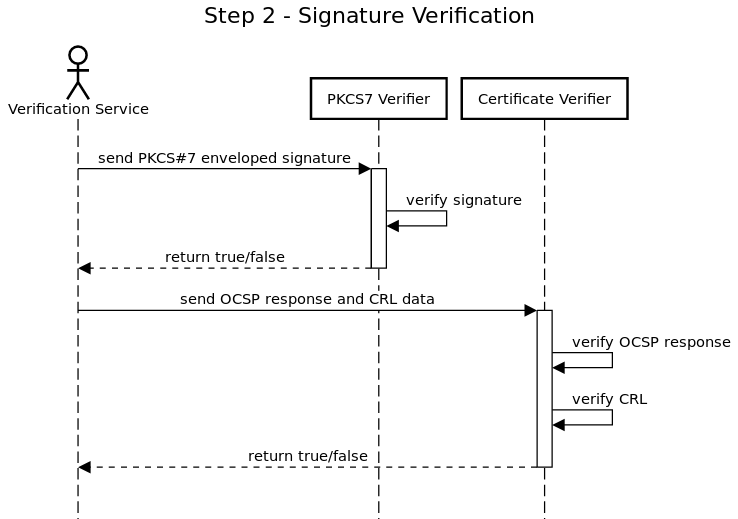
\includegraphics[scale=0.5]{images/protocol_verification_step2_signature.png}
        \caption{Signature verification step}
        \label{fig:signatureverificationstep}
    \end{center}
\end{figure}

Then, the ID token itself needs to be verified,
as well as the certificate chain of the key used to sign the ID token (figure~\ref{fig:idtokenverification}).

\begin{figure}
    \begin{center}
        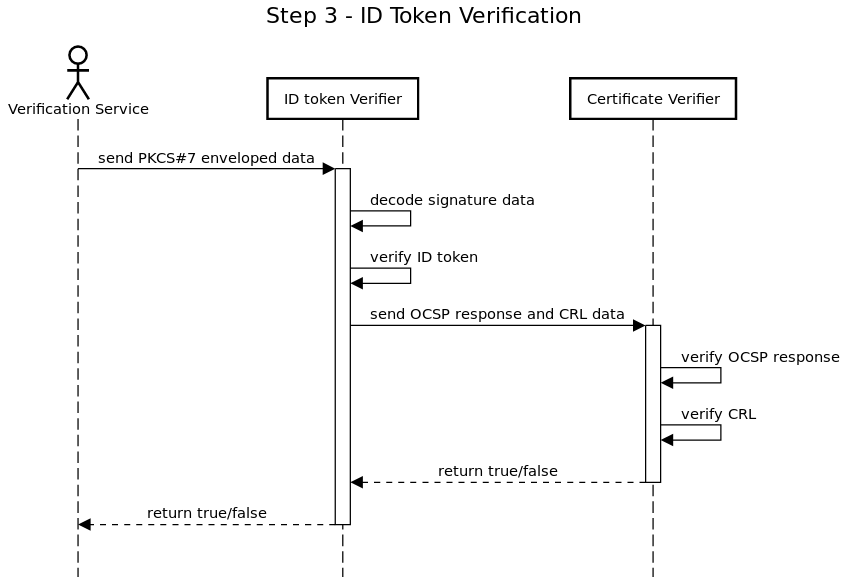
\includegraphics[scale=0.5]{images/protocol_verification_step3_id_token.png}
        \caption{ID token verification}
        \label{fig:idtokenverification}
    \end{center}
\end{figure}

In order to verify the link of the document hashes with the ID token,
the document hash needs to be salted, inserted into the sorted list of the other salted hashes,
and the resulting list hashed again.
The result must be the same as the nonce in the ID token.
At last, the hash of the document must match the included hash.
Figure~\ref{fig:signaturedataverification} illustrates this process.

\begin{figure}
    \begin{center}
        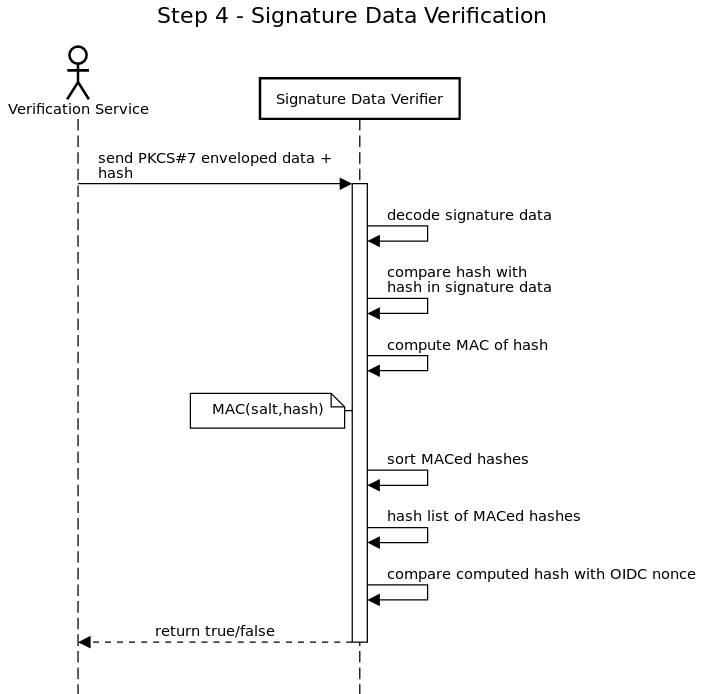
\includegraphics[scale=0.5]{images/protocol_verification_step4_signature_data.png}
        \caption{Signature data verification}
        \label{fig:signaturedataverification}
    \end{center}
\end{figure}

\section{REST API}\label{sec:rest-api}
In this section the \gls{REST} \gls{API} is specified:
Which endpoints are offered, what they expect as input data and what they respond with.
The examples are given for illustration purposes and are not normative.

\subsection{Signing Service}
The signing service offers the following endpoints:

\begin{longtable}{|l|l|l|l|}
    \hline
    \textbf{No.} & \textbf{Endpoint} & \textbf{Method} & \textbf{Description} \\ \hline
    1 & /api/v1/login & POST & Send hashes to sign, receive list of OIDC providers \\ \hline
    2 & /api/v1/sign & POST & Send hashes to sign, receive signature URL \\ \hline
    3 & /api/v1/signatures/:id & GET & Retrieve signature file \\ \hline
    \caption{Endpoints offered by the Signing Service}
\end{longtable}

In the most common case, the client application will call these endpoints in the order listed:
\begin{enumerate}
    \item The user submits the hashes of the documents they wish to sign and receives a list of IDPs
    \item After authentication with the IDP, the user submits the hashes again, this time the server will begin construction of the signature file
    \item After the signature is created, the user downloads the file to their device
\end{enumerate}

But, the order in which these endpoints are used is not enforced by the API except for what is required with the \gls{OIDC} implicit flow,
and the linkage of the id\_token with the signing.

\subsubsection{Client errors}
\label{apiclienterrors}
If a malformed request is sent by the client, the signing server will respond with a 400 client error code,
and a message indicating the cause of failure.
This format of returning errors is the same for all endpoints of the signing server.

\begin{longtable}{|l|l|l|l|}
    \hline
    \textbf{Parameter} & \textbf{Presence} & \textbf{Type} & \textbf{Description} \\ \hline
    message & MANDATORY & String & Reason for rejection of request \\ \hline
    \caption{Output in case of invalid input}
\end{longtable}

Sample Error Response:
\begin{lstlisting}[caption={Error response}, captionpos=b, language=JavaScript, label={lst:errorresponse}]
    HTTP/1.1 400 Bad Request
    Content-Type: application/json

    {
    "message": "Invalid hash length"
    }
\end{lstlisting}

\subsubsection{login}
This endpoint is used for submitting the hashes the user wishes to sign.

\begin{longtable}{|l|l|l|l|}
    \hline
    \textbf{Parameter} & \textbf{Presence} & \textbf{Type} & \textbf{Description} \\ \hline
    hashes & MANDATORY & List<String> & Hashes of the documents to be signed \\ \hline
    \caption{Input to the login endpoint}
\end{longtable}

Duplicates in the list of hashes are not allowed and are rejected by the API as described in~\ref{apiclienterrors}.
The length of each hash is checked, and if they don't match the hashing algorithm used the request is rejected as well.
The encoding of the hashes is checked, and if they don't appear to be a string of sane hex numbers the request is rejected.

Output:

\begin{longtable}{|l|l|l|l|}
    \hline
    \textbf{Parameter} & \textbf{Presence} & \textbf{Type} & \textbf{Description} \\ \hline
    providers & MANDATORY & Map<String, Url> & List of providers with the redirect url \\ \hline
    seed & MANDATORY & String & Seed for generating the salt \\ \hline
    salt & MANDATORY & String & Salt for generating the OIDC nonce \\ \hline
    \caption{Output of the login endpoint}
\end{longtable}

Sample Request:
\begin{lstlisting}[caption={login request}, captionpos=b, language=JavaScript, label={lst:hashesrequest}]
    POST /api/v1/hashes HTTP/1.1
    Host: service.example.org
    Content-Type: application/json

    {
    "hashes": [
    "e8a96e6203b9c0df058ba862abc63d9c520157faef6d5d54e54e526b0a85b2be",
    "0b9a7fd3e612061a7fe6d834e102a143170f33d0e8c5a8eb79416aa3eb53c0d6"
    ]
    }
\end{lstlisting}

Sample Response:
\begin{lstlisting}[caption={login response}, captionpos=b, language=JavaScript, label={lst:hashesresponse}]
    HTTP/1.1 201 Created
    Content-Type: application/json

    {
    "providers": {
    "SwissID": "https://...&nonce=6cd7ef99e5e79d68d681e5d097b7f805381c4d013152fa3f26d06bd728ae49fa",
    "Google": "https://...&nonce=6cd7ef99e5e79d68d681e5d097b7f805381c4d013152fa3f26d06bd728ae49fa"
    },
    "seed": "84c97acc49335faa0266fb29b4228205e9400a85a10faa68ec30cf894e1730ed",
    "salt": "cfb663431af5e2d68be48867f93e86e477cd7eeefc10b16a51c238d2c810561b"
    }
\end{lstlisting}

\subsubsection{sign}\label{subsubsec:signrequest}
After having authenticated with the IDP, the client application calls the signing endpoint.
This is where the actual signature file is being assembled by the signing server.

\begin{longtable}{|l|l|l|l|}
    \hline
    \textbf{Parameter} & \textbf{Presence} & \textbf{Type} & \textbf{Description} \\ \hline
    id\_token & MANDATORY & string & OIDC ID token \\ \hline
    seed & MANDATORY & String & Seed for generating the salt \\ \hline
    salt & MANDATORY & String & Salt for generating the OIDC nonce \\ \hline
    hashes & MANDATORY & List<String> & Hashes of the documents to be signed \\ \hline
    \caption{Input to the signing endpoint}
\end{longtable}

The signing server performs the checks described in \ref{subsubsec:verificationhashesseedsalt},
and if any of them fail to pass,
the server rejects the request as described in~\ref{apiclienterrors}.

Output:

\begin{longtable}{|l|l|l|l|}
    \hline
    \textbf{Parameter} & \textbf{Presence} & \textbf{Type} & \textbf{Description} \\ \hline
    signature url & MANDATORY & Url & Url to the generated signature file\\ \hline
    \caption{Output of the signing endpoint}
\end{longtable}

Sample Request:
\begin{lstlisting}[caption={sign request}, captionpos=b, language=JavaScript, label={lst:signrequest}]
    POST /api/v1/sign HTTP/1.1
    Host: service.example.org
    Content-Type: application/json

    {
    "id\_token": {...},
    "seed": "84c97acc49335faa0266fb29b4228205e9400a85a10faa68ec30cf894e1730ed",
    "salt": "cfb663431af5e2d68be48867f93e86e477cd7eeefc10b16a51c238d2c810561b",
    "hashes": [
        "e8a96e6203b9c0df058ba862abc63d9c520157faef6d5d54e54e526b0a85b2be",
        "0b9a7fd3e612061a7fe6d834e102a143170f33d0e8c5a8eb79416aa3eb53c0d6"
        ]
    }
\end{lstlisting}

Sample Response:

\begin{lstlisting}[caption={sign response}, captionpos=b, language=JavaScript, label={lst:signresponse}]
    HTTP/1.1 201 Created
    Content-Type: application/json

    {
        "signature": "https://signingservice.local/api/v1/signatures/0b1131ca0b68f3d55b8e32a55e8"
    }
\end{lstlisting}

\subsubsection{signatures/:id}
Input:

\begin{longtable}{|l|l|l|l|}
    \hline
    \textbf{Parameter} & \textbf{Presence} & \textbf{Type} & \textbf{Description} \\ \hline
    id & MANDATORY & String & id of the hash that was signed \\ \hline
    \caption{Input to the signature retrieval endpoint}
\end{longtable}

Output: Binary data, meant to be presented to the user as a file download


Sample Request:

\begin{lstlisting}[caption={signature request}, captionpos=b, language=JavaScript, label={lst:signaturerequest}]
    GET /api/v1/signatures/e8a96e62034e526b0a85b2be HTTP/1.1
    Host: service.example.org
\end{lstlisting}

Sample Response:

\begin{lstlisting}[caption={signature response}, captionpos=b, language=JavaScript, label={lst:signatureresponse}]
    HTTP/1.1 200 OK
    Content-Type: application/octet-stream
    Content-Disposition: attachment; filename="signaturefile"

    <binary data follows>
\end{lstlisting}

\subsection{Verification Service}
Endpoints:

\begin{longtable}{|l|l|l|}
    \hline
    \textbf{Endpoint} & \textbf{Method} & \textbf{Description} \\ \hline
    /api/v1/verify & POST & Send hash signature file for verification \\ \hline
    \caption{Overview of endpoints offered by the verification service}
\end{longtable}

\subsubsection{verify}
Input:

\begin{longtable}{|l|l|l|l|}
    \hline
    \textbf{Parameter} & \textbf{Presence} & \textbf{Type} & \textbf{Description} \\ \hline
    hash & MANDATORY & String & Hash of the signed document \\ \hline
    signature & MANDATORY & String & base64 encoded signature file \\ \hline
    \caption{Input to the signature verification endpoint}
\end{longtable}

Output:

\begin{longtable}{|l|l|l|l|}
    \hline
    \textbf{Parameter} & \textbf{Presence} & \textbf{Type} & \textbf{Description} \\ \hline
    valid & MANDATORY & Boolean & validity of signature \\ \hline
    error & OPTIONAL & String & error message why the signature is invalid \\ \hline
    id\_token & MANDATORY & Object & id token + claims + cert chain \\ \hline
    signature & MANDATORY & Object & signature data (hashes, salt, algorithms) \\ \hline
    signing\_cert & MANDATORY & Object & cert chain of signer cert + signer info \\ \hline
    timestamp & MANDATORY & Object & signing time and cert chain \\ \hline
    \caption{Output of the signature verification endpoint}
\end{longtable}

Sample Request:
\begin{lstlisting}[caption={sign request}, captionpos=b, language=JavaScript, label={lst:verifyrequest}]
    POST /verify HTTP/1.1
    Host: service.example.org
    Content-Type: application/json

    {
    "hash": "e8a96e6203b9c0df058ba862abc63d9c520157faef6d5d54e54e526b0a85b2be",
    "signature": "IyMjIFJFU1QgQVBJIFNwZWNpZmljYXRpb24gU2NyYXRjaHBhZAoKIyMjIyBQcmUtQXV0aCBlbmRw...b2ludCAKIyMjIyMgRW5kcG9pbnQKYGBgUE9TVCAvYXBpL3YxL3NpZ25gYGAK"
    }
\end{lstlisting}

Sample Response:

\lstinputlisting[caption={Sign response}, captionpos=b, language=JavaScript, label={lst:verifyresponse}]{listings/verifyResponse.txt}

Invalid signature:

\begin{lstlisting}[caption={sign response}, captionpos=b, language=JavaScript, label={lst:verifyresponsefailed}]
    HTTP/1.1 200 OK
    Content-Type: application/json

    {
    "valid": false,
    "error": "signed hash and provided hash don't match"
    }
\end{lstlisting}

\section{Signature File Format}\label{sec:signature-file-format}
Digital signatures unfortunately aren't very simple.
Several components have to be put together for them to work.
TODO better introduction, explain why so many components are needed.
\subsection{High-Level Overview}\label{subsec:high-level-overview}
The signature file consists of the following parts, from innermost to outermost:

\begin{itemize}
    \item The innermost part of the signature file is the information that is being signed.
    \item This information gets enveloped in a RFC~5652~\cite{rfc5652} \gls{CMS} message along with certificates and revocation information.
    \item This \gls{CMS} is encoded with \gls{DER}\footnote{We like to think of DER encoding as in German, "DER ENCODING!", the one and only encoding! We thought it was funny.} and added to a Protobuf message.
    \item A number RFC~3161~\cite{rfc3161} timestamps are added to the same Protobuf message.
\end{itemize}

In the following subsections each of these parts is explained in more detail.

\subsection{SignatureData: The information that is being signed}\label{subsec:signaturedata:-the-information-that-is-being-signed}
The information that is being signed is structured as a Protobuf message with the following schema:

\begin{lstlisting}[caption={SignatureData schema}, captionpos=b, label={lst:signaturedataschema}]
message SignatureData {
    repeated bytes salted_document_hash = 1;
    HashAlgorithm hash_algorithm = 2;
    bytes mac_key = 3;
    MACAlgorithm mac_algorithm = 4;
    SignatureLevel signature_level = 5;
    bytes id_token = 6;
    bytes jwk_idp = 7;
    map<string, LTV> ltv_idp = 8;
}
\end{lstlisting}

\paragraph{salted\_document\_hash} is a list of salted document hashes.
The are salted as described in section~\ref{subsec:pre-login}.
There must be at least one salted hash.
There cannot be more than 100'000 hashes.
We limit this so that no one tries encoding arbitrary data in there (like pictures of cats) just because they can.

\paragraph{hash\_algorithm} is the hash algorithm used for the values in \texttt{salted\_document\_hash} as well as the \gls{OIDC} nonce.
\paragraph{mac\_key} is the key fed to the \gls{HMAC} function specified by \texttt{mac\_algorithm} for masking the hashes.
For an explanation on that masquerade and why it's done see~\ref{subsec:pre-login}.
\paragraph{mac\_algorithm} is the specific \gls{HMAC} function that's being used to masquerade the hashes.
\texttt{mac\_key} is the key that's fed to \texttt{mac\_algorithm}.
\paragraph{signature\_level} is either qualified or advanced, depending on the \gls{LoA} provided by the \gls{IDP}.
For an explanation on what advanced and qualified signatures are, see~\ref{subsec:difference-between-advanced-and-qualified-signatures}.
\paragraph{id\_token} is the \gls{OIDC} token issued by the \gls{IDP}.
It must be included into the signature file in order for the verifier to be able to confirm that the user authenticated with the \gls{IDP},
the linkage between the document hashes submitted to the \gls{IDP}, the authentication and the signature file.
If this token weren't included the signing server could issue signatures on its own, which we're making impossible.
\paragraph{jwk\_idp} is the \gls{JWK} according to RFC~7517~\cite{rfc7517} as published by the \gls{IDP}.
It is included for verification of the signature on the \texttt{id\_token}.
\paragraph{ltv\_idp} envelops \gls{CRL} and \gls{OCSP} information for the certificates in the \gls{CA} chain of the certificate used by the \gls{IDP} when signing the \gls{OIDC} \texttt{id\_token}.
This separate protobuf message is necessary because contrary to \gls{CMS}, the \gls{JWK} specification~\cite{rfc7517} doesn't allow for including revocation information.
Because there may be a number of certificates in the \gls{JWK}, this field is a map of the fingerprint of the certificate to its revocation information.
The field is optional, it's only needed if \gls{LTV} is desired.
For more information on \gls{LTV} see~\ref{subsec:long-term-validation}.

\paragraph{Putting it together}

These fields are put into the protobuf message \texttt{SignatureData} (for the schema, see listing~\ref{lst:signaturedataschema}).
The message is serialised to its binary format.
Then, a \gls{CMS} message is constructed, enveloping and signing the binary-serialised \texttt{SignatureData} protobuf message.
The signer certificate along with the \gls{CA} certificate chain is added to the \gls{CMS} message, and if \gls{LTV} is desired,
their respective \gls{CRL} and \gls{OCSP} responses.

Please note that RFC~5652~\cite{rfc5652} \gls{CMS} messages are required and no older standards
because they don't allow for including \gls{OCSP} responses, only \gls{CRL}s.
For more information on including \gls{OCSP} in \gls{CMS} see~\cite[Section 10.2.1, RevocationInfoChoices and OtherRevocationInfoFormat]{rfc5652}.

In summary, we now have serialised the core signature information, signed it, and combined it with certificate information.
The next step is to timestamp the signature as described in~\ref{subsec:signaturefile:-combining-signed-data-with-timestamps}.

\subsection{SignatureFile: Combining signed data with timestamps}\label{subsec:signaturefile:-combining-signed-data-with-timestamps}
All signatures issued by the signing server are augmented by at least one timestamp by at least one \gls{TSA} independent of the signing server and the \gls{IDP}.

\subsubsection{Why timestamp?}
Timestamping allows the verifier to assert the point in time the signature was created.
This information is confirmed by a party independent of the signature service and the \gls{IDP},
thus the verifier can be fairly confident about the authenticity of this information.

It's important for the verifier to know reliably when the signature was created,
because that way the verifier is able to check whether the certificates used where valid at the time of signature creation,
not at signature validation time.

Someone could ask, why not just put the date and time of creation into the signature itself?
It would be much simpler and easier,
instead of going through the trouble of obtaining one or more RFC~3161~\cite{rfc3161} timestamps
from independent trusted third parties.
If the date and time were part of the signed data it would be protected by the digital signature,
and no one would be able to alter it.

That's not good enough, because we need to guard against \gls{CA} failure.
Imagine what happened if the \gls{CA} used by the signing server were compromised:
all certificates issued by that \gls{CA} would get revoked,
and thus all signatures created with these certificates would become invalid.
Potentially millions of contracts and other such documents would become effectively null and void in an instant,
with widespread and quite possibly disastrous repercussions on its users
(like losing a house, because from a legal perspective, the mortgage has just disappeared into thin air).
All information authenticated by certificates signed by that \gls{CA} would become untrustworthy,
including the date and time of creation included in it.

Fortunately, in our solution, it is highly unlikely that someone is able to forge a signature even if they
completely compromised the \gls{CA}, because they'd need to compromise the \gls{IDP} or its \gls{CA} as well
in order to be able to falsify a signature.

But even so, all issued signatures becoming void is unacceptable.

This is why the timestamping is so important.
The timestamp confirms that the signatures were issued before the \gls{CA} was compromised,
thus protecting their validity.
This is also the reason why the signing server can't just add the date and time of creation in the signature on its own,
because that information is protected by a signature that was created with a certificate authenticated
by a compromised \gls{CA}, thus making that information useless.

By using at least one independent third party \gls{TSA} the time of signature creation can be ascertained,
because that information is authenticated by a different \gls{CA}.
The risk can be reduced further by combining \gls{TSA}s.
Then the signature will remain valid even if the signature server \gls{CA} and the \gls{TSA} \gls{CA} were compromised.

Readers knowledgeable with \gls{JWT} will observer that we could use the \texttt{iat} (Issued At) and \texttt{exp} (Expiration Time)
claims from the \texttt{id\_token} issued by the \gls{IDP} instead of adding a RFC~3161~timestamp,
since the \texttt{id\_token} is signed by a party using a different \gls{CA} than the signing server as well,
but unfortunately these claims are optional and we can't rely on them being present~\cite[Sections 4.1.4 and 4.1.6]{rfc7519}.

There's another reason for using timestamps: \glsdesc{LTV}; but this is out of scope for this chapter.
For more information on that please refer to~\ref{subsec:long-term-validation}.

\subsubsection{Combining the SignatureData CMS with the RFC~3161 timestamps}
For adding the timestamp(s) to the \gls{CMS} message created in~\ref{subsec:signaturedata:-the-information-that-is-being-signed}
we define another Protobuf message as follows:

\begin{lstlisting}[caption={SignatureFile message}, captionpos=b, label={lst:signaturefileschema}]
message SignatureFile {
    bytes signature_data = 1;
    repeated bytes rfc3161 = 2;
}
\end{lstlisting}

\paragraph{signature\_data} is the \gls{DER}-encoded \gls{CMS} message created as described in~\ref{subsec:signaturedata:-the-information-that-is-being-signed}.
\paragraph{rfc3161} is one or more \gls{DER}-encoded timestamps according to RFC~3161~\cite{rfc3161}.

Any number of timestamps can be added.
Timestamps either confirm \texttt{signature\_data} or another timestamp earlier in the chain.
The chains of timestamps that are formed that way can be used for \gls{LTV} as described in~\ref{subsec:long-term-validation}.

The signature file returned to the user is the binary serialisation of \texttt{SignatureFile}.


\subsection{Long-Term Validation}\label{subsec:long-term-validation}
\glsdesc{LTV} allows for the validation of signatures long after the document was signed~\cite{etsipades}.

We need \gls{LTV} for two main reasons:
\begin{enumerate}
    \item Imagine if the \gls{CA} were revoked that was used for the signatures: all signatures created using the same \gls{CA} would become invalid instantly, making countless documents, constracts and the like unverifiable.
    \item Extending the validity of the signature beyond the lifetime of the \gls{CA} used to sign it, for signatures that need to remain valid and verifiable for a very long time.
\end{enumerate}
In order for us to achieve this, all required elements for signature validation must be embedded into the signature file.
Without the addition of these elements, a signature can only be validated for a limited time.
This limitation occurs because the \gls{CA}s eventually expire, or get revoked.
Once the \gls{CA} certificate has expired, the issuing authority is no longer responsible for providing the revocation status information on that certificate.
Without the confirmed revocation status information on the signing keys, the signature cannot be validated.

To overcome this limitation, the following information has to be embedded into the signature:
\begin{enumerate}
    \item A timestamp on the signature
    \item The signing certificate
%    \item The certificates used and their revocation status (\gls{OCSP} and \gls{CRL})
    \item An archive timestamp of the previous content
\end{enumerate}

The archive timestamp establishes the date in which the information collected was issued.
Provided the archive timestamp is valid,
we can be sure that the revocation information was issued at that time,
and check the validity of the signing certificate and the \gls{CA} certificate chain.
Thus we can be certain that it was not revoked at the point in time the document was signed.
This allows us to extend the validity of the signature past the expiration time of the \gls{CA}.

However, this does not extend the validity of the signature indefinitely,
it merely extends the expiration until the expiration time of the timestamping authority's certificate.

For many cases this may be enough, but it doesn't quite allow for long-time archival yet.
When the timestamping certificates' expiration is impending,
the signature expiration time has to be extended by adding another timestamp signed by a \gls{CA} not yet close to expiration.
This re-stamping has to be repeated periodically in order to keep the signature valid and verifiable.
This allows for near-indefinite archival.

